\documentclass[main.tex]{subfiles}
 
\begin{document}
\chapterimage{band1.jpg}
\chapter{Remote Control (Cloud)}

The true potential for smart connected devices can be realised when the connectivity is used to control or monitor the device remotely, or through integration with other services. This is where the cloud communication comes into picture. In this Chapter, we will get the connected to a cloud platform, and enable remote control and monitoring of the device.

Typically, this is achieved through either of the scenarios as shown in the figure \ref{fig:cloud_connectivity}.

\begin{figure}
    \centering
    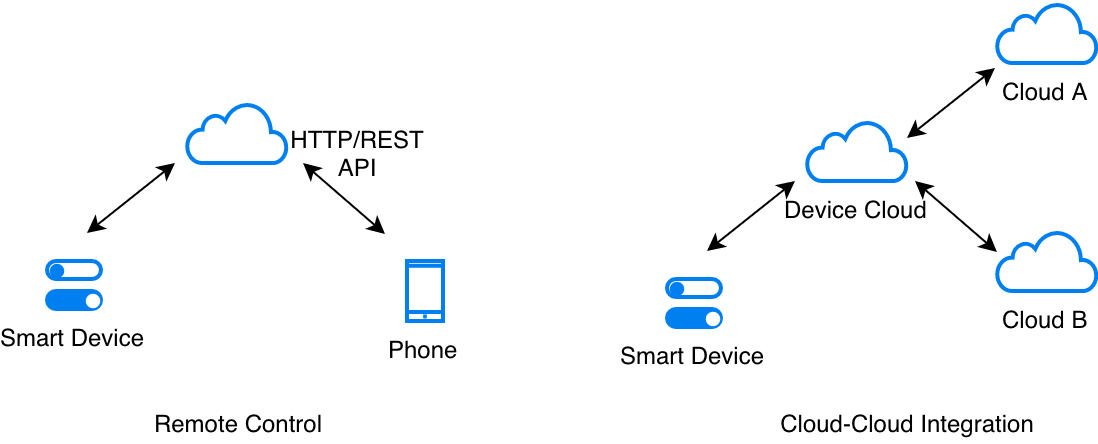
\includegraphics[scale=0.4]{../../_static/cloud_connectivity.png}
    \caption{Value of Cloud Connectivity}
    \label{fig:cloud_connectivity}
\end{figure}

In most cases, once a device is connected to the cloud, the Device Cloud platforms expose the device control and monitoring through a RESTful web API. Authenticated clients, like smartphone apps can use these APIs to access the device remotely.

Additionally, integration with other clouds also helps in realising valuable use cases. For example, the device can be linked with a weather information system to automatically tune itself, or it can be linked to voice-assistant cloud interfaces (like Alexa or Google Voice Assistant) to expose control through voice.

\section{Security First}\index{Security First}\label{sec:security_first}
Before we get into the details about cloud connectivity, a few important words about security. 

Connecting with any remote cloud infrastructure must always happen using TLS (Transport Layer Security). It is a standard and it takes care of ensuring that communication stays secure. This is a transport layer protocol. Any higher-level protocols like HTTP, or MQTT can use TLS as the underlying transport. All reputable cloud vendors provide device services over TLS.

\subsection{CA Certificates}\index{CA Certificates}
One aspect of TLS is server validation using CA certificates. The TLS layer uses the CA certificate to validate that you are really talking to the server that you are supposed to talk to. For this validation to happen, your device must be pre-programmed with one or more valid and trusted CA certificate. The TLS layer will use these as trusted certificates and then validate the server based on these trusted certificates. Please refer to Section \ref{sec:embedding_files} for more details about how the CA certificate be made part of your firmware.

\subsection{Additional Details}\index{Additional Details}

More details about TLS and certificates is available at: \url{https://medium.com/the-esp-journal/esp32-tls-transport-layer-security-and-iot-devices-3ac93511f6d8}

\section{Embedding Files in the Firmware}\index{Embedding Files in the Firmware}\label{sec:embedding_files}
At times, the firmware has to use certain files directly. Most commonly, in the case of CA certificates, that need to be embedded within the firmware for server validation.

The question is how do you make the entire contents of these files be part of your firmware image, and how do you access them within your firmware?

ESP-IDF provides a great mechanism for enabling this. The \textit{component.mk} file can be used to inform the build system that the contents of certain files should be embedded within firmware image. This can be enabled by adding the following line into your application's \textit{component.mk} file.

\begin{minted}{cmake}
COMPONENT_EMBED_TXTFILES := certs/server-root-ca.pem 
\end{minted}

In the above example, the build system will make the file \textit{certs/server-root-ca.pem} be part of the firmware. The contents of this file are in the firmware's address space and can be directly addressed as follows:
\begin{minted}{c}
extern const uint8_t certificate_pem_crt_start[] asm("_binary_server_root_ca_start");
extern const uint8_t certificate_pem_crt_end[] asm("_binary_server_root_ca_end");
\end{minted}

The file can then be accessed using these start and end pointers.

\section{AWS IoT}\index{AWS IoT}\label{sec:aws_cloud}
In this section we will connect the device to Amazon's AWS IoT cloud. 

\subsection{Quick Setup}\index{Quick Setup}
XXX Specify quick setup instructions

\subsection{Demo}\index{Demo}
By the end of the previous sub-section, you should have the following items ready to get your device to start talking with AWS IoT:
\begin{enumerate}
    \item A Device Private Key (a file)
    \item A Device Certificate (a file)
    \item A Thing Name (a string)
    \item A CA Certificate for the AWS-IoT service's domain name (a file)
\end{enumerate}

Before getting into the details of the code, let us actually try to use the remote control for our device.
You may refer to the \textit{4cloud/} directory of esp-jumpstart for trying this out.

To setup your AWS IoT example, 
\begin{enumerate}
    \item Go to the \textit{5\_cloud/} application
    \item Copy the files (overwriting any previous files) as mentioned below:
    \begin{itemize}
        \item The AWS CA Certificate to \textbf{5\_cloud/certs/aws-root-ca-.pem}
        \item The Device Private Key to \textbf{5\_cloud/certs/private.pem.key}
        \item The Device Certificate to \textbf{5\_cloud/certs/certificate.pem.crt}
    \end{itemize}
    \item Modify the thing name \textbf{EXAMPLE\_THING\_NAME} in the file \textit{5\_cloud/main/cloud.c}
    \item Build, flash and load the firmware on your device
\end{enumerate}

The firmware is so written that it will now connect to the AWS IoT cloud platform and will notify the cloud of any state changes. The firmware will also fetch any updates to the state from the cloud and apply them locally. 

\subsection{Remote Control}\index{Remote control}
For remote control, AWS IoT exposes a RESTful web API for all devices that connect to it. Phone applications can interact with this Web API to control and monitor the device. We will use cURL, a command-line utility that can be used to simulate this phone app. 

Using curl, we can then read the current state of the device by executing the following command on your Linux/Windows/Mac console:
\begin{minted}{console}

curl --tlsv1.2 --cert /work/certificate.pem.crt \
       --key /work/private.pem.key   \
       https://aln7lww42a72l-ats.iot.us-east-2.amazonaws.com:8443/things/my_device_name/shadow \ 
       | python -mjson.tool

\end{minted}

AWS expects that access to a device state is only granted to entities that are authorised to do so. Hence in the command above, we use the \textit{certificate.pem.crt} and \textit{private.pem.key}, which are the same files that we have configured to be in the firmware. This ensures that we can access the device's state.

In the command above, this reads the state from the device \textbf{my\_device\_name}. Don't forget to replace this with the name of your thing.

The device state can be modified as:
\begin{minted}{console}

curl -d '{"state":{"desired":{"output":false}}}' \ 
     --tlsv1.2 --cert /work/certificate.pem.crt \ 
     --key /work/private.pem.key \ 
     https://aln7lww42a72l-ats.iot.us-east-2.amazonaws.com:8443/things/my_device_name/shadow \ 
     | python -mjson.tool
\end{minted}

This cURL command will generate an HTTP POST operation, and sends the JSON data, as shown above, as the post's body. This JSON data instructs AWS IoT to update the state of the device to false.

You can observe the corresponding change of state on the device whenever you change the state from cURL to true or false.

So that's how remote control is achieved. Let's now quickly talk about the code.

\subsection{The Code}\index{The Code}
All the code for the cloud communication has been consolidated in the \textit{cloud.c} file. The structure of this file is similar to what the standard AWS IoT SDK expects.

The file uses our output driver's APIs, \textit{app\_driver\_get\_state()} and \textit{app\_driver\_toggle\_state()}, to fetch and modify the device state respectively.

The AWS IoT requires 3 files to be embedded within your firmware:
\begin{itemize}
        \item The AWS CA Certificate  \textbf{5\_cloud/certs/aws-root-ca-.pem}
        \item The Device Private Key  \textbf{5\_cloud/certs/private.pem.key}
        \item The Device Certificate  \textbf{5\_cloud/certs/certificate.pem.crt}
\end{itemize}
The application uses the mechanism as shown in Section \ref{sec:embedding_files} for embedding this within the firmware.

\section{Progress so far}\index{Progress so far}
With this application we finally tie the functionality of the device (outlet power toggle) to network connectivity. Connecting it to the cloud makes it now accessible to be controlled and monitored over the network. We also looked at the security aspects that we must consider before connecting to any remote/cloud service.

As our next step, let's look at one of the most common requirements of a connected device, the over-the-air (OTA) firmware upgrade.
\end{document}
